\begin{anexos}
	\subsubsection{Prompts Utilizados}
	\subsubsection{-Preprocesamiento}
	\begin{lstlisting}
	Analiza la información del dataframe y define las tareas de preprocesamiento necesarias.
	Considera:
	- Conversión de fechas a datetime.
	- Identificación de columnas categóricas.
	- Sugerencias para filtrar columnas no numéricas no categóricas.
	
	```json
	[
	{"tarea": "convertir_fecha", "columna": "nombre_columna"},
	{"tarea": "identificar_categorica", "columna": "nombre_columna"},
	{"tarea": "filtrar", "columna": "nombre_columna", "sugerencia": "sugerencia filtro para la columna, puede ser simplemene eliminar la columna, eliminar filas con datos faltantes o filtrar valores outliers"}
	{"tarea": "pandas","codigo":"codigo pandas para realizar el procesado del dataframe almacenado en df, este se ejecuta para realizar una tarea mas compleja, que no sea convertir_fecha,identificar_categorica,o filtrar"}
	]
	```
	Ademas sugiere 3 posibles consultas que un usuario que esta analizando el dataframe pueda hacerse del mismo
	
	--IMPORTANT--
	ANSWER FORMAT
	<Analisis de que datos tienes y que se deberia hacer>
	```json
	<json array con las tareas>
	```
	A continuacion se muestran 3 sugerencias de consultas
	```sugerencia
	<Sugerencia de una consulta que pueda realizar el usuario sobre los datos del dataframe>
	```
	```sugerencia
	<Sugerencia 2 de una consulta>
	```
	```sugerencia
	<Sugerencia 3>
	```
	\end{lstlisting}
	
	\subsubsection{-Corrección de Errores en el código python.}
	\begin{lstlisting}
		You generated Python code that produced an error. Please debug and regenerate the corrected code. There are a df variable with the dataframe already defined, and libraries pandas as pd and altair as alt are available
		Original code:\n```python\n{original_code}\n```\nError message: {error_message}\nCorrected code:
	\end{lstlisting}
	
	\subsubsection{-Generar Esqueleto}
	\begin{lstlisting}
		Dada la siguiente consulta del usuario sobre el documento cargado, genera un esqueleto detallado para un reporte que pueda responder a la consulta de forma exhaustiva. El esqueleto debe estructurar la información de manera lógica y facilitar la creación de un reporte final completo.
		
		DOCUMENT INFORMATION
		{st.session_state.document_info}
		
		ANSWER FORMAT:
		[Un analisis del tema y de lo que quiere el usuario, de que datos quiere conocer, y que datos extras podrian proporcionarsele para una respuesta mas completa]
		[Analisis de la consulta, Identificar los puntos clave de la consulta (qué información busca el usuario explícitamente), Identificar posibles ambigüedades o interpretaciones de la consulta, Definir las métricas o datos específicos necesarios para responder a la consulta]
		<Esturctura del Reporte>
		```json
		[
		'section': {{
				'name':[Nombre de la seccion del reporte]
				'description':[Breve descripcion de la seccion del reporte]
				'data':[brevemente el tipo de información que se va a incluir (ej: "Datos de ventas del producto A", "Gráfico comparativo", "Conclusiones") Indicar si se requieren visualizaciones (gráficos, tablas), y en caso afirmativo, sugerir tipos apropiados (ej: "Gráfico de barras para comparar ventas", "Tabla con datos numéricos detallados")]
				'extra_data':[Sugerir información adicional o contextual que pueda enriquecer la respuesta y aportar mayor valor al usuario (datos relevantes que no se solicitaron explícitamente pero podrían ser útiles)]
		}},
		{{"section": {{
						"name": "[Nombre de la siguiente sección]",
						"description": "[Descripción de la siguiente sección]",
						"data": "[Tipo de información y visualización]",
						"extra_data":"[información adicional para esta sección]"
				}}
		}},...
		]
		```
		
		EXAMPLE
		User Input: Comparar las ventas del producto A y B en el último trimestre.
		
		ANSWER:
		
		```json
		[
		{{
				"section": {{
						"name": "Introducción",
						"description": "Breve contexto del reporte de ventas y mención de la comparación solicitada de los productos A y B. Objetivo del reporte: analizar y comparar el rendimiento de ventas de ambos productos.",
						"data": "Contexto general del análisis de ventas",
						"extra_data": "Mencionar la relevancia de comparar estos productos para la estrategia de la empresa"
				}}
		}},
		{{
				"section": {{
						"name": "Datos de Ventas del Producto A (último trimestre)",
						"description": "Presentación detallada de las ventas del Producto A en el último trimestre",
						"data": "Datos numéricos de ventas. Sugerencia: Tabla detallada",
						"extra_data": "Comparación de ventas de A con trimestres anteriores."
				}}
		}},
		{{
				"section": {{
						"name": "Datos de Ventas del Producto B (último trimestre)",
						"description": "Presentación detallada de las ventas del Producto B en el último trimestre",
						"data": "Datos numéricos de ventas. Sugerencia: Tabla detallada",
						"extra_data": "Comparación de ventas de B con trimestres anteriores."
				}}
		}},
		{{
				"section": {{
						"name": "Gráfico Comparativo de Ventas (A vs B)",
						"description": "Comparación visual de las ventas de A y B",
						"data": "Gráfico de barras para comparar ventas. Sugerencia: Gráfico de barras",
						"extra_data":"Comparación de porcentajes de crecimientos"
				}}
		}},
		{{
				"section": {{
						"name": "Tabla Comparativa de Ventas (A vs B)",
						"description": "Tabla con datos comparativos detallados de A y B",
						"data": "Tabla con datos numéricos y porcentajes. Sugerencia: Tabla detallada",
						"extra_data": "Datos de ventas por región"
				}}
		}},
		{{
				"section": {{
						"name": "Conclusiones y Análisis",
						"description": "Análisis de los resultados y conclusiones del reporte",
						"data": "Resumen de los hallazgos y conclusiones.",
						"extra_data": "Mencionar limitaciones o posibles investigaciones futuras."
				}}
		}}
		]
		```
	\end{lstlisting}
	
	\subsubsection{-Obtener el código python para la extración de datos.}
	\begin{lstlisting}
		Teniendo en cuenta los datos del documento siguiente se te ha pedido que generes una seccion de un reporte.
		Tu trabajo es solo generar la parte textual de la seccion, para ello necesitas informacion extra, a la cual puedes acceder usando codigo python
		sobre el siguiente documento, el cual se encuentra en un dataframe de pandas llamado "df".
		DOCUMENT INFORMATION
		{st.session_state.document_info}
		
		ANSWER GUIDE
		Los datos que desees recibir al final se deben encontrar en una variable local llamada "response" con una estrucutra de datos adecuada como por ejemplo json.
		Si deseas recibir varios datos como por ejemplo valor maximo y minimo de una columna de un dataframe, debes incluirlos todos en la variable "response".
		Ten en cuenta de que solo la informacion que necesitas es solo para la parte textual de la seccion del reporte por lo que si quieres ver por ejemplo como se comportaron
		las ventas de un año en cuestion, no debes incluir toda la informacion de la base de dato con respecto a las ventas de ese año ya que para el reporte escrito
		son demasiados datos, solo debes incluir en la respuesta la informacion importante que puedas sacar con codigo python de estas como maximos minimos media, outlier,
		patrones etc.
		Solo debes proporcionar un codigo python con todas las instrucciones necesarias para obtener la toda la informacion requerida de una.
		NO PUEDES MODIFICAR EL DATAFRAME ORIGINAL ALMACENADO EN "df".
		
		En caso de que no necesites informacion del dataframe
		
		ANSWER FORMAT:
		<Analisis de que datos necesitas conocer para la seccion>
		```python
		<CODIGO PYTHON>
		```
		"""
	\end{lstlisting}
	
	\subsubsection{-Generar el código python para la obtención de gráficos.}
	\begin{lstlisting}
		Teniendo en cuenta los datos del documento siguiente se te ha pedido que generes una o varias graficas o tablas sobre el siguiente documento, el cual se encuentra en un dataframe de pandas llamado "df".
		DOCUMENT INFORMATION
		{st.session_state.document_info}
		
		ANSWER GUIDE
		Las graficas o tablas que generes debes ser en codigo altair, libreria que ya esta importada como 'import altair as alt'.
		Las graficas o tablas que desees recibir al final se deben encontrar en una variable local llamada "response" el cual debe ser una lista de graficas o tablas altair.
		cada elemento de la lista debe ser un diccionario con la siguiente estructura:
		{{
				'name':<nombre_del_grafico>,
				'description':<breve descripcion de que datos muestra este grafico>,
				'c':<objeto altair>
		}}
		
		Ten en cuenta de que solo necesitas las graficas especificas para la seccion actual del reporte, las graficas mas generales son para las secciones de conclusiones o alguna que la requiera especificamente.
		
		Solo debes proporcionar un codigo python con todas las instrucciones necesarias para obtener todas las graficas requerida de una.
		NO PUEDES MODIFICAR EL DATAFRAME ORIGINAL ALMACENADO EN "df".
		
		En caso de que la seccion no requiera graficas haz que el codigo python devuelva uen response sea una lista vacia
		
		ANSWER FORMAT:
		<Analisis de que graficos o tablas serian ilustrativos en esta seccion>
		```python
		<CODIGO PYTHON>
		```
	\end{lstlisting}
	
	\subsubsection{-Generar y estructurar el informe final.}
	\begin{lstlisting}
		Teniendo en cuenta los datos del documento siguiente se te ha pedido que generes una seccion de un reporte.
		
		DOCUMENT INFORMATION
		{st.session_state.document_info}
		
		ANSWER GUIDE
		Para generar el reporte lo mas certero posible se te brindan los siguientes datos:
		
		{response}
		
		Genera la seccion del reporte con la informacion proporcionada, utiliza esos datos para cumplir con las espectativas del reporte en la seccion actual.
		
		Para complementar tu respuesta tienes a tu dispocision los siguientes graficos o tablas
		{charts_names}
		
		Los cuales puedes incluir en tu reporte donde los cosideres oportuno usando la siguiente sintaxis
		```chart
		<chart_name>
		```
		No es necesario mostrar algun o todos los graficos si estos no son relevates para la seccion actual.
		
		ANSWER FORMAT:
		<Texto del reporte>
		```chart
		<nombre del grafico a insertar>
		```
		<Pude seguir el texto del reporte, incluir otro grafico a continuacion o intercalarlos en dependencia de lo que requiera esta seccion del reporte>
	\end{lstlisting}
	
	\subsubsection{Ejemplo de un reporte completo generado}
	\begin{figure}[H]
		\centering
		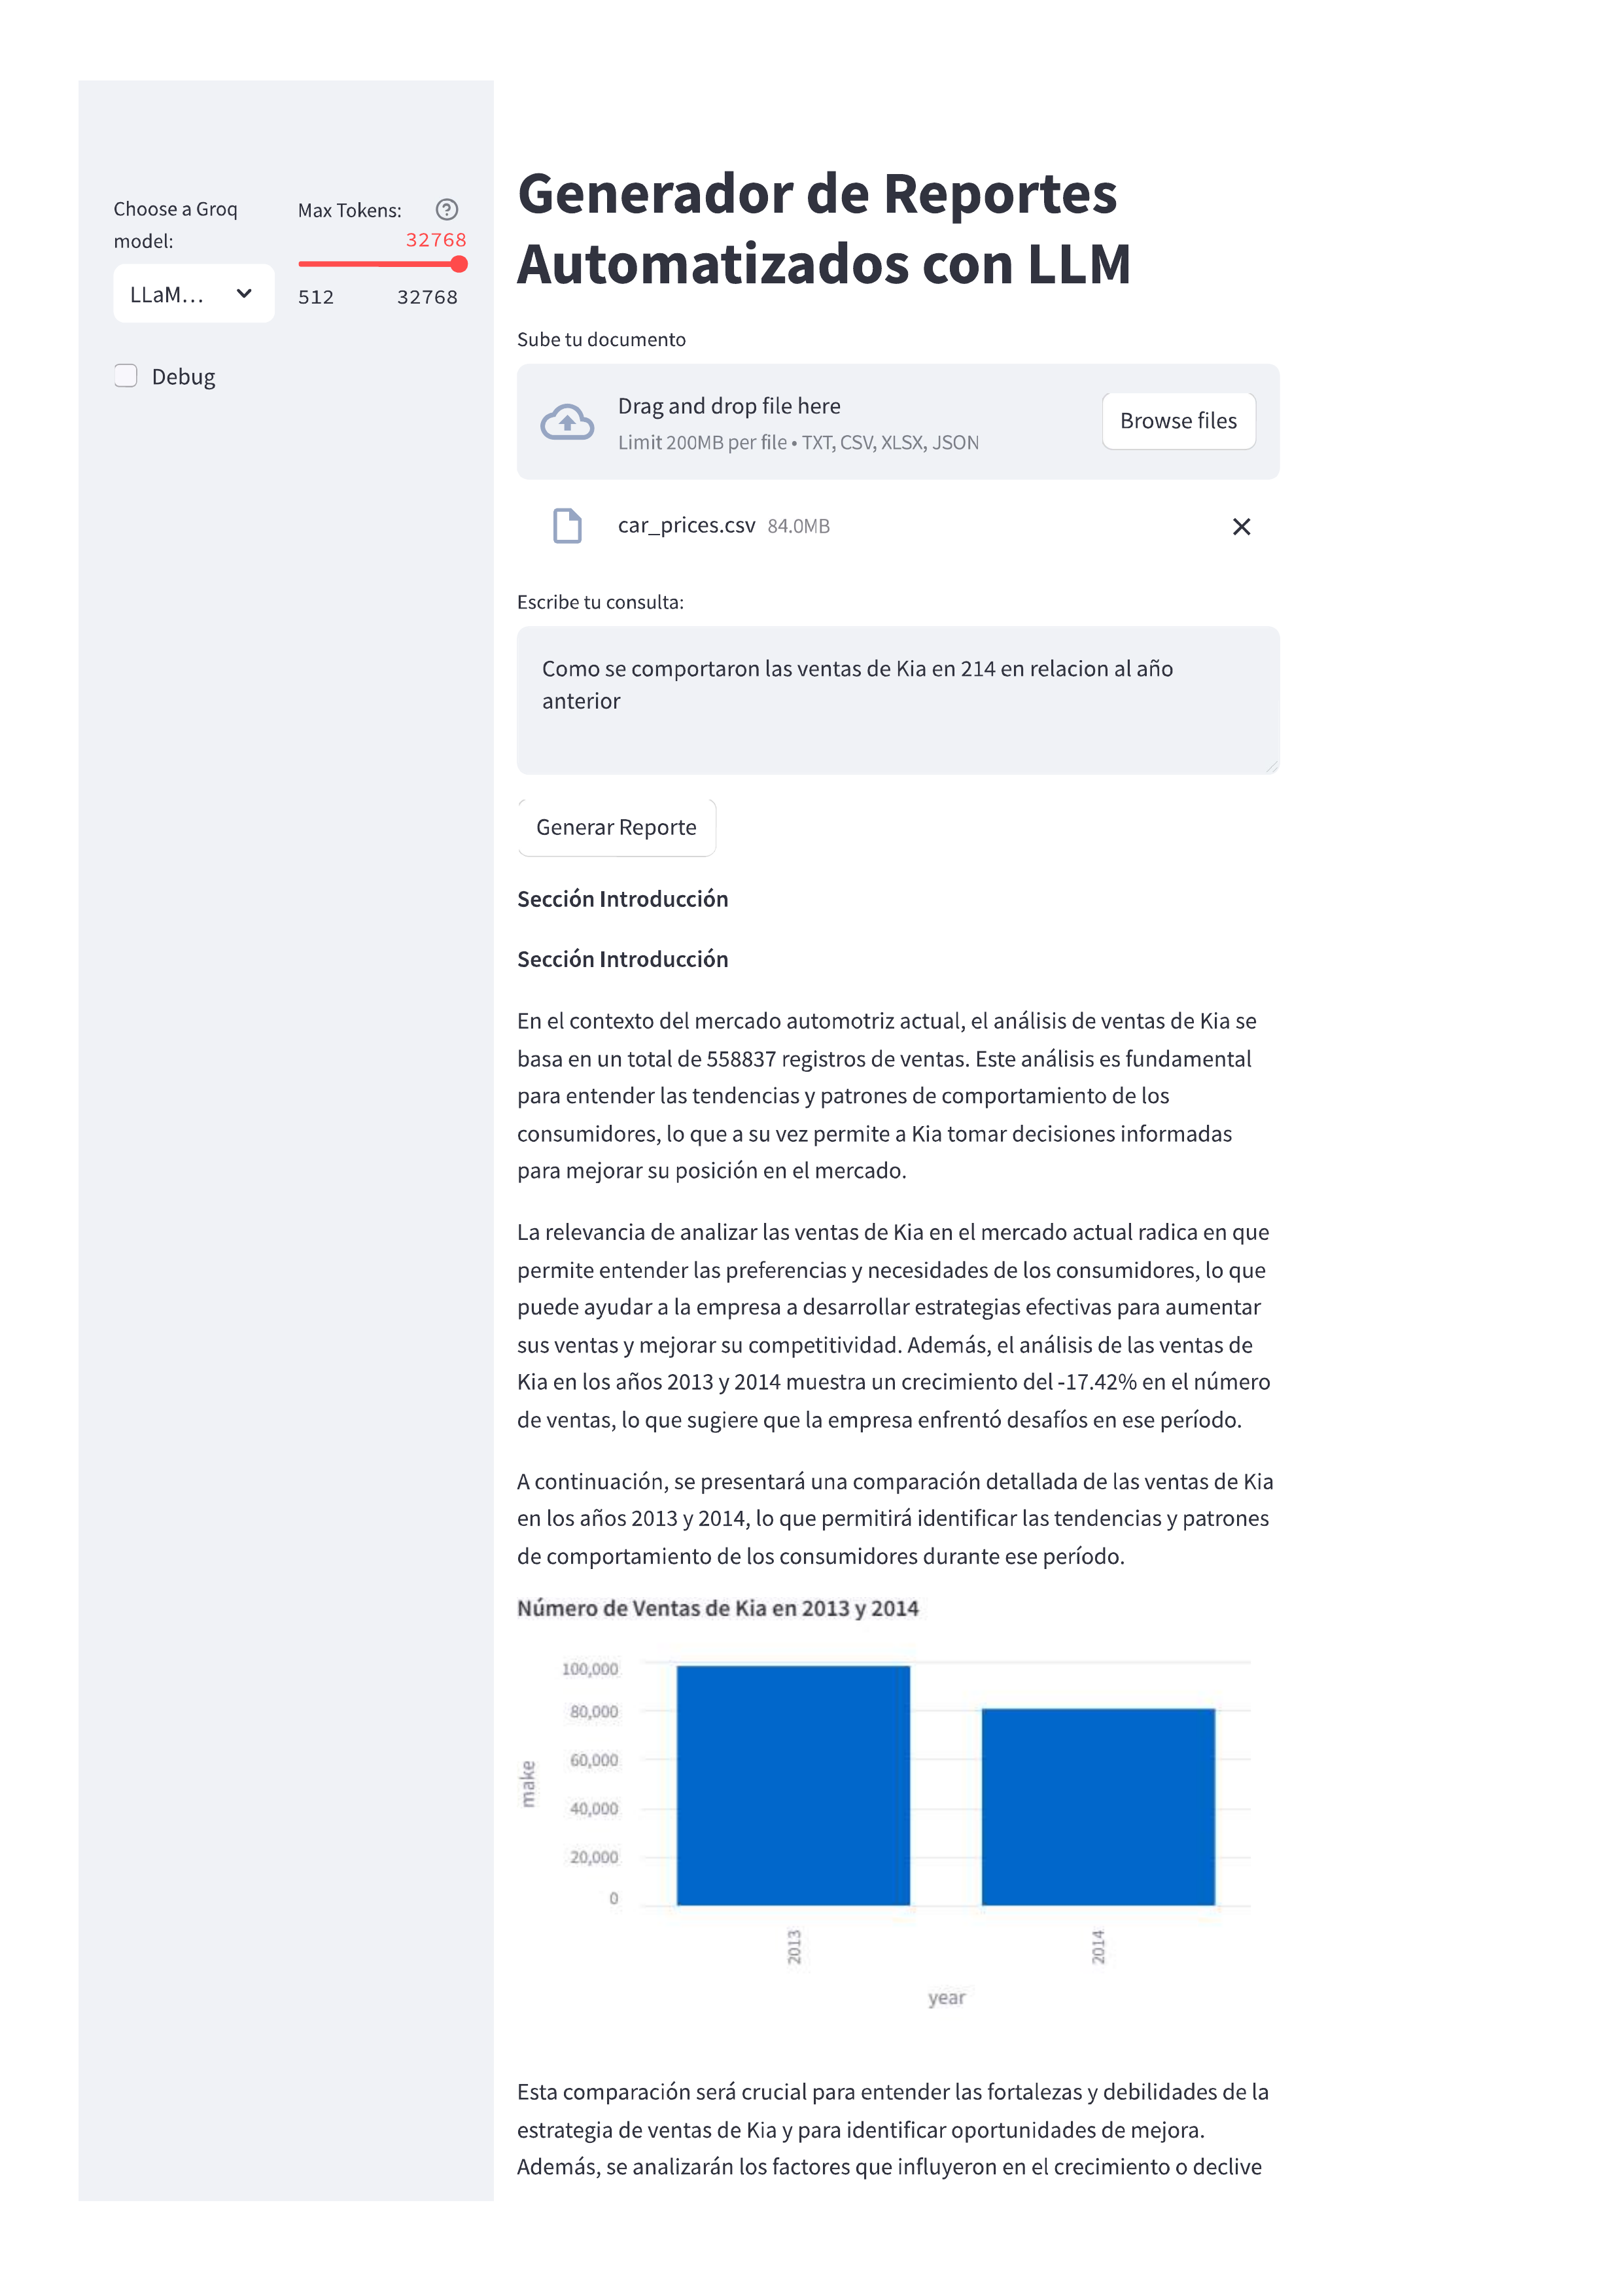
\includegraphics[height=\textheight]{reporte/1.png}
	\end{figure}
	\begin{figure}
		\centering
		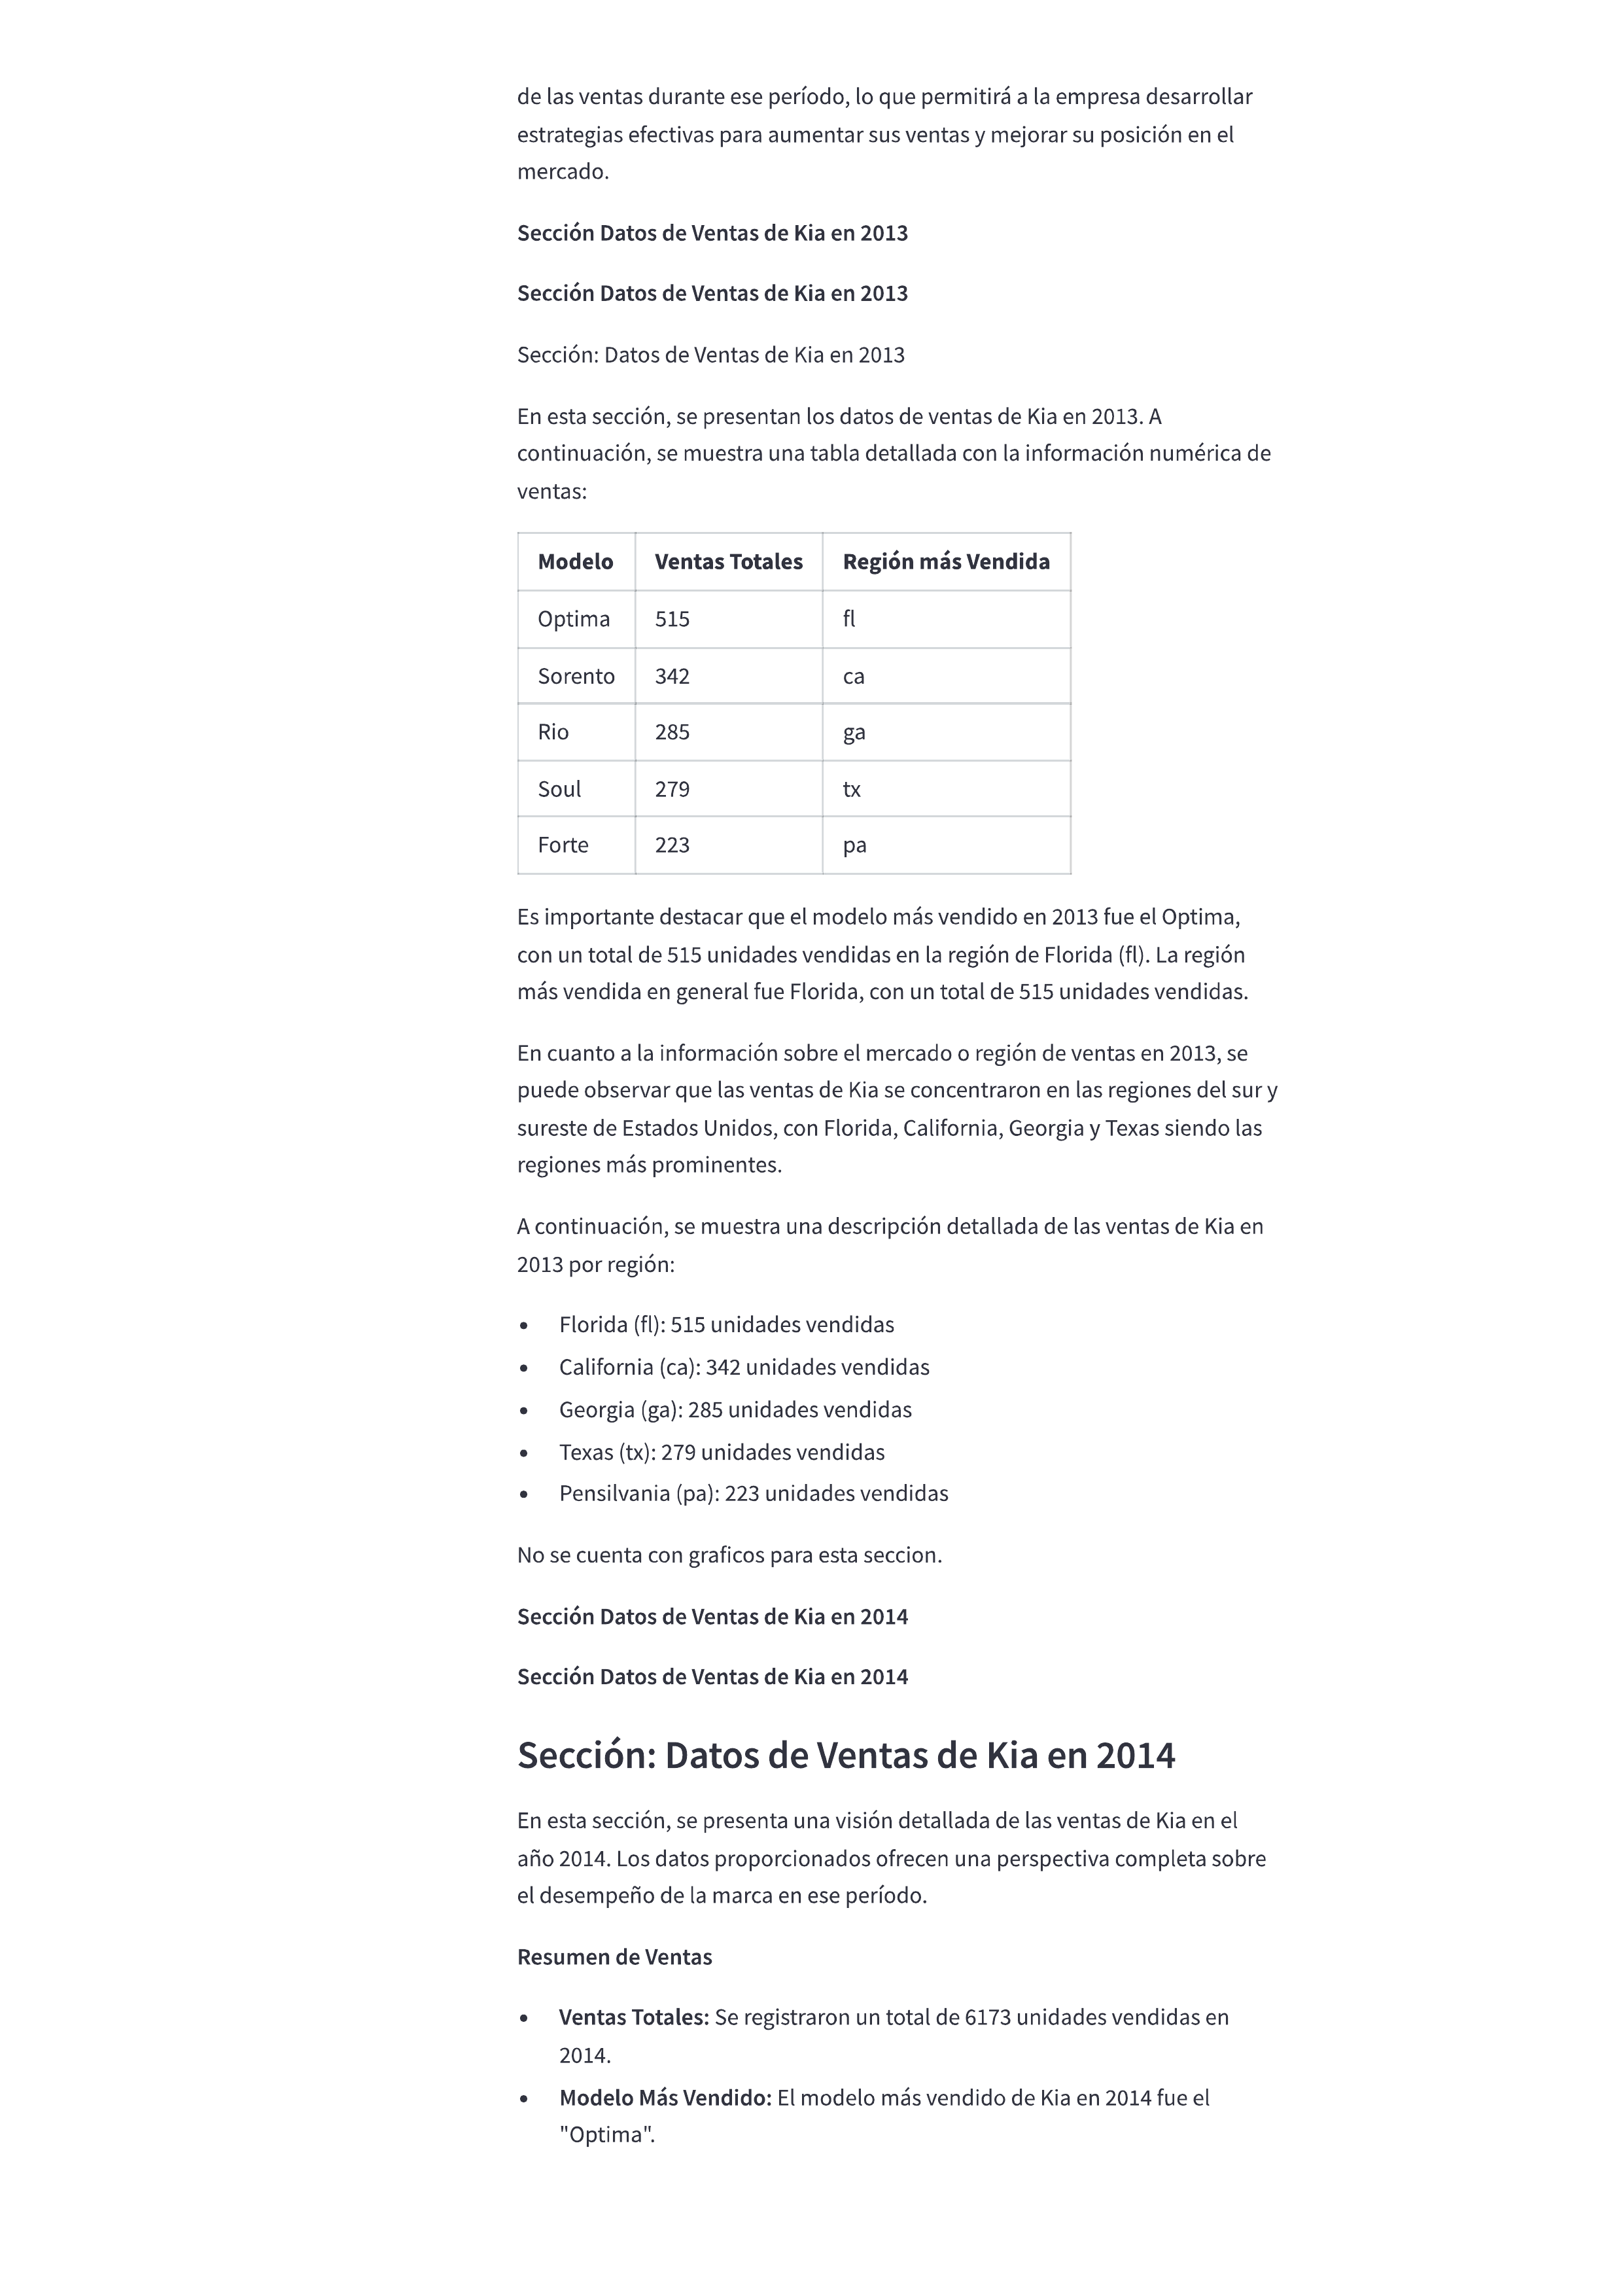
\includegraphics[height=\textheight]{reporte/2.png}
	\end{figure}
	\begin{figure}
		\centering
		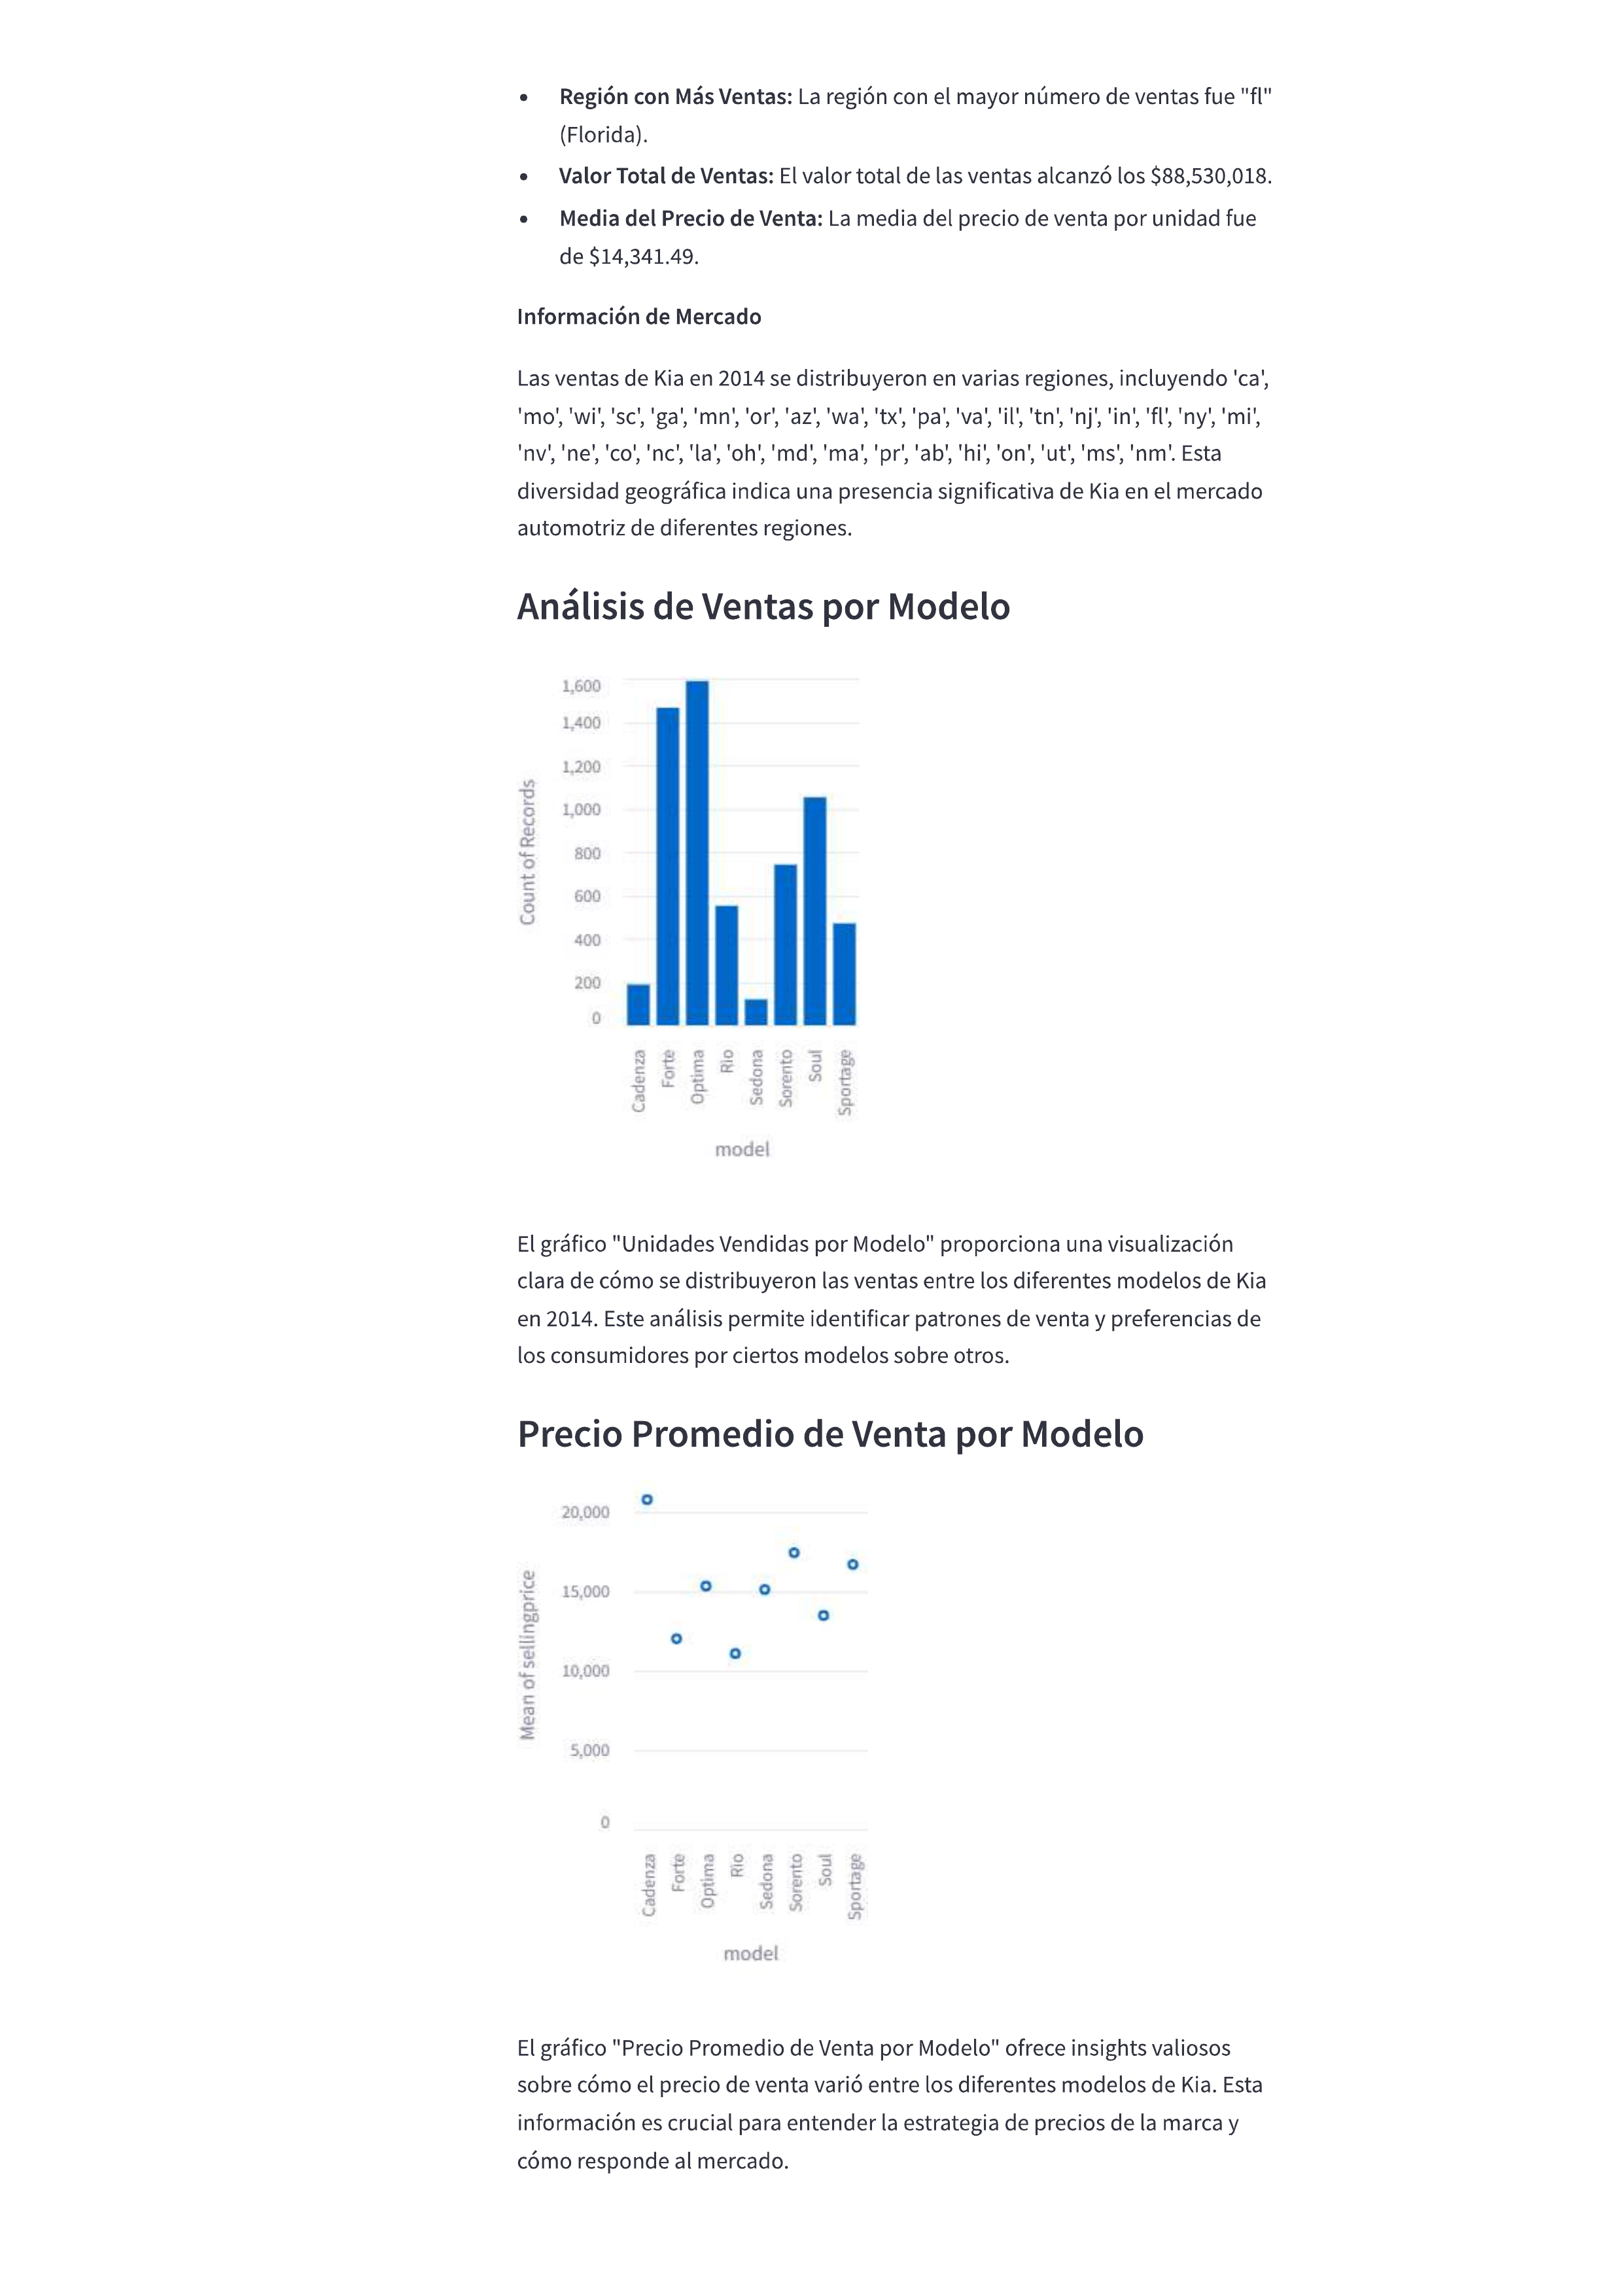
\includegraphics[height=\textheight]{reporte/3.png}
	\end{figure} 
	\begin{figure}
		\centering
		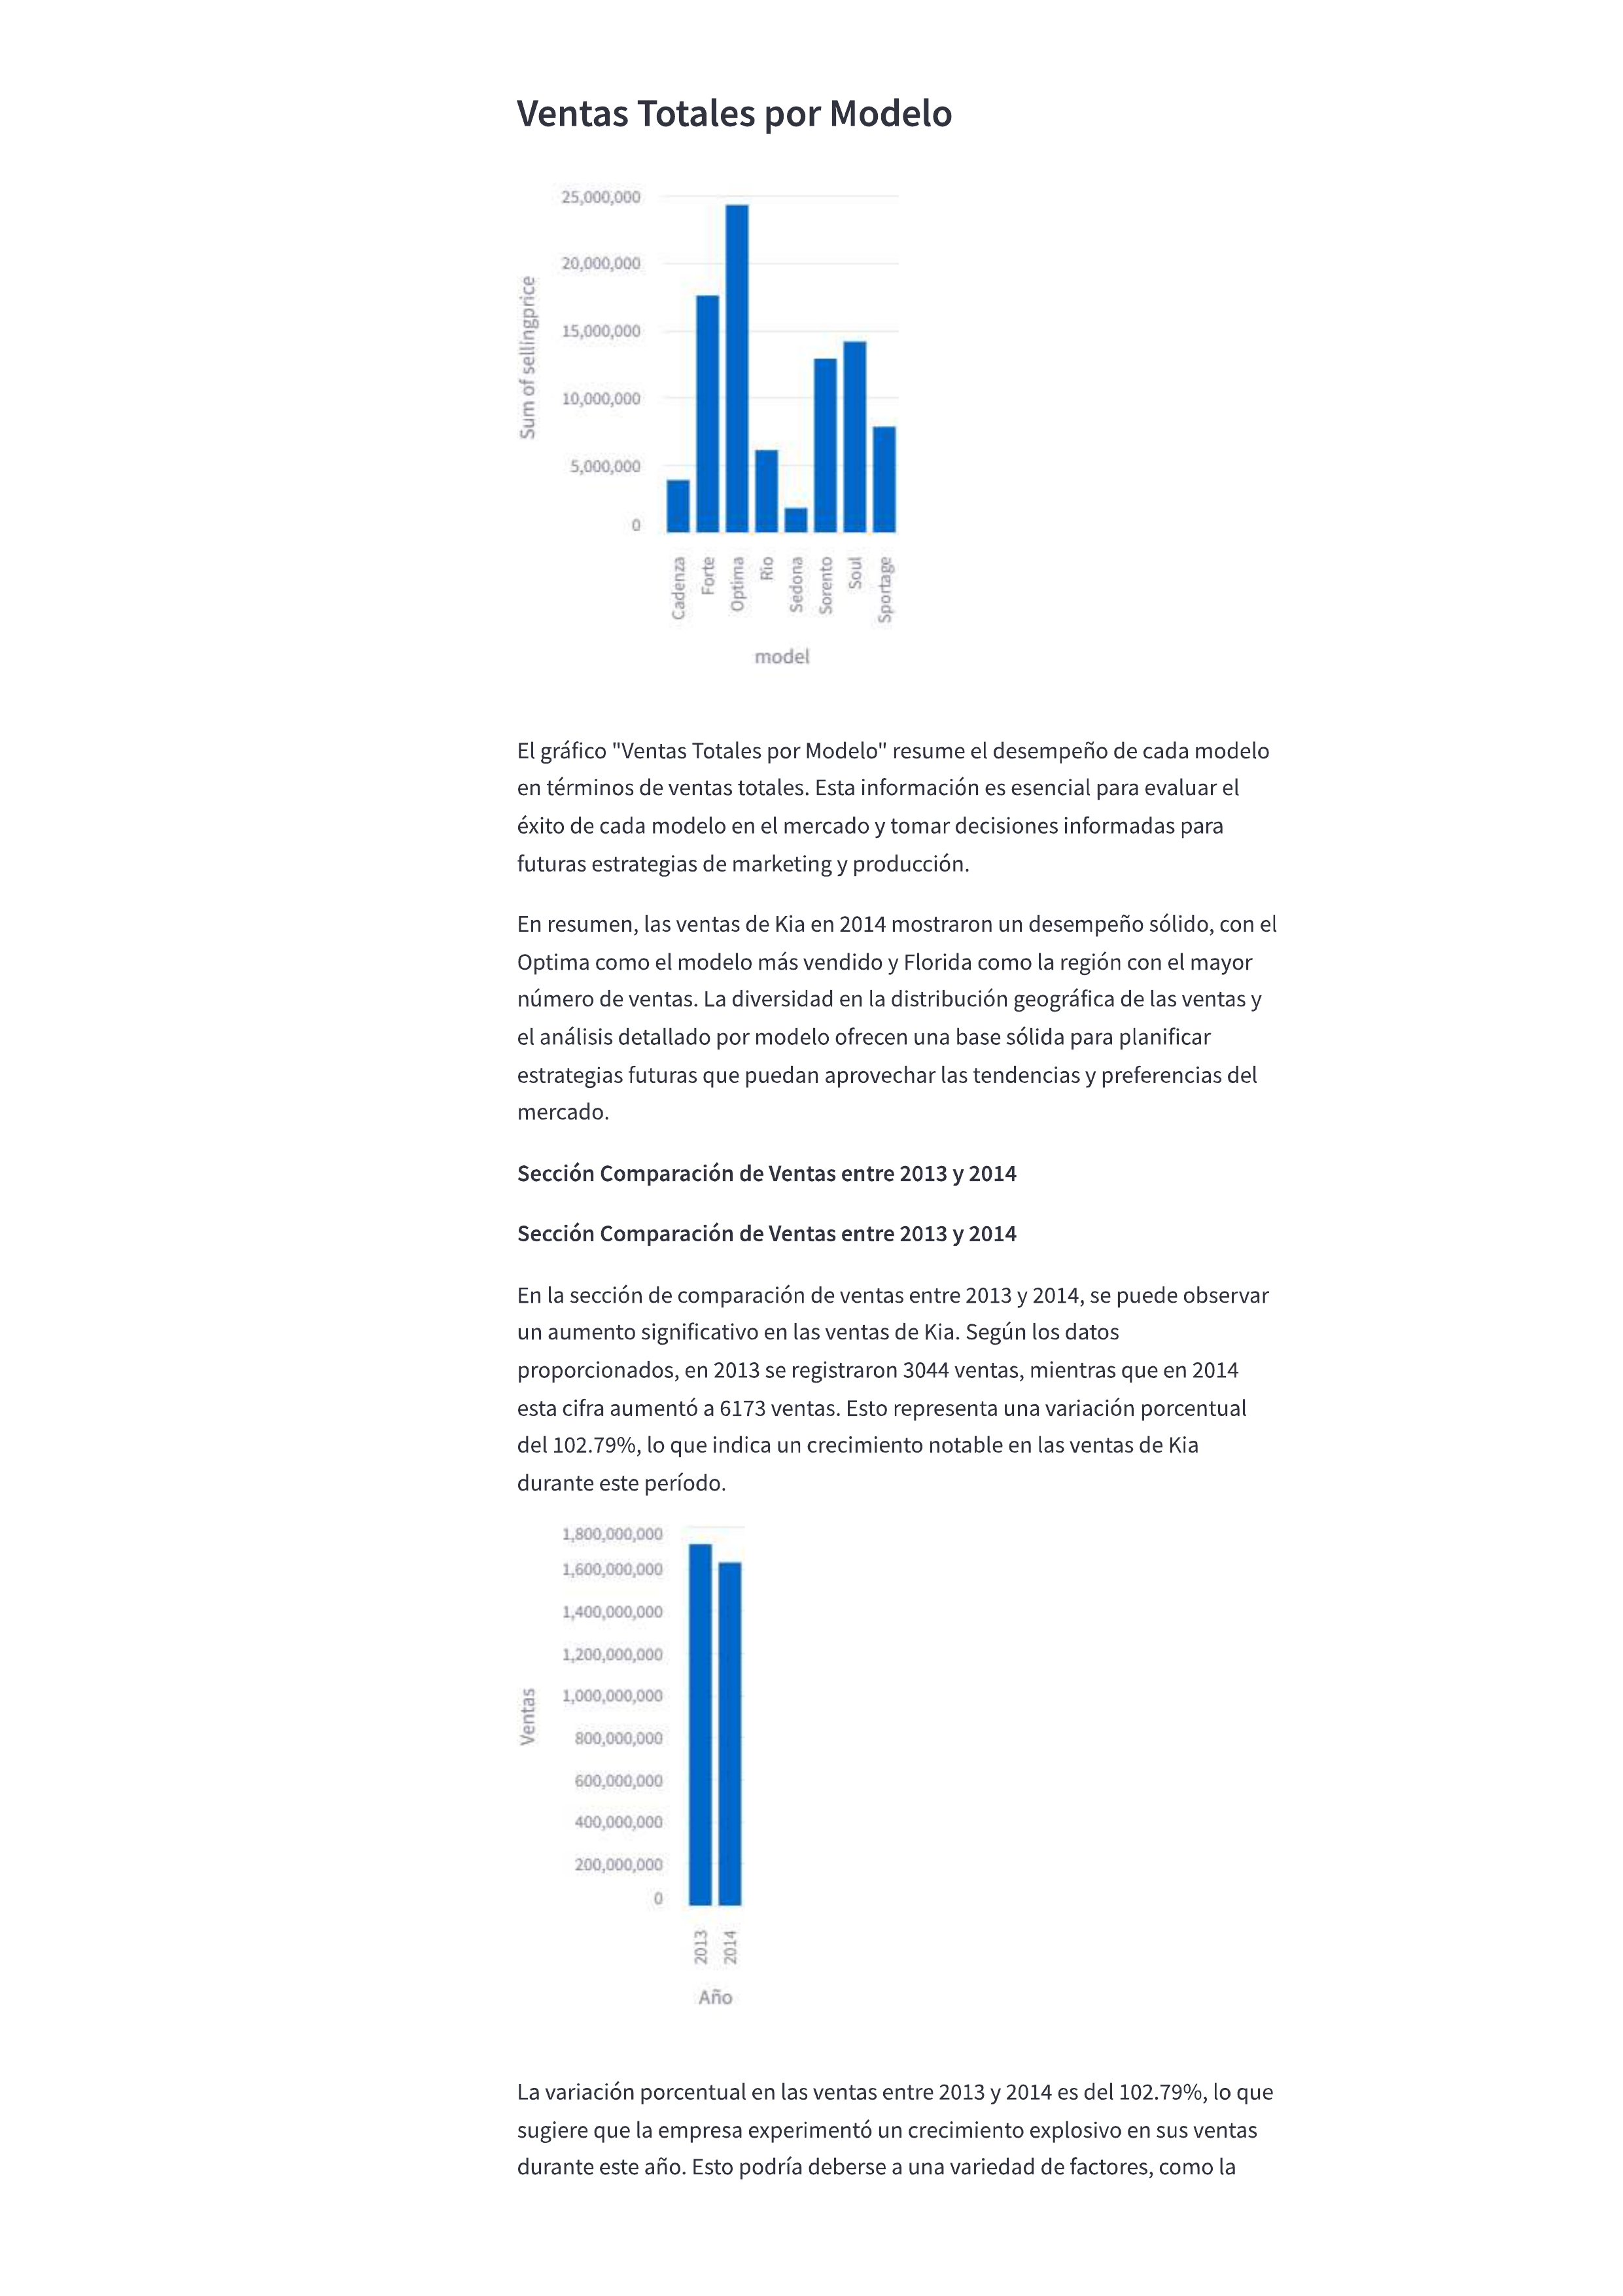
\includegraphics[height=\textheight]{reporte/4.png}
	\end{figure}
	\begin{figure}
		\centering
		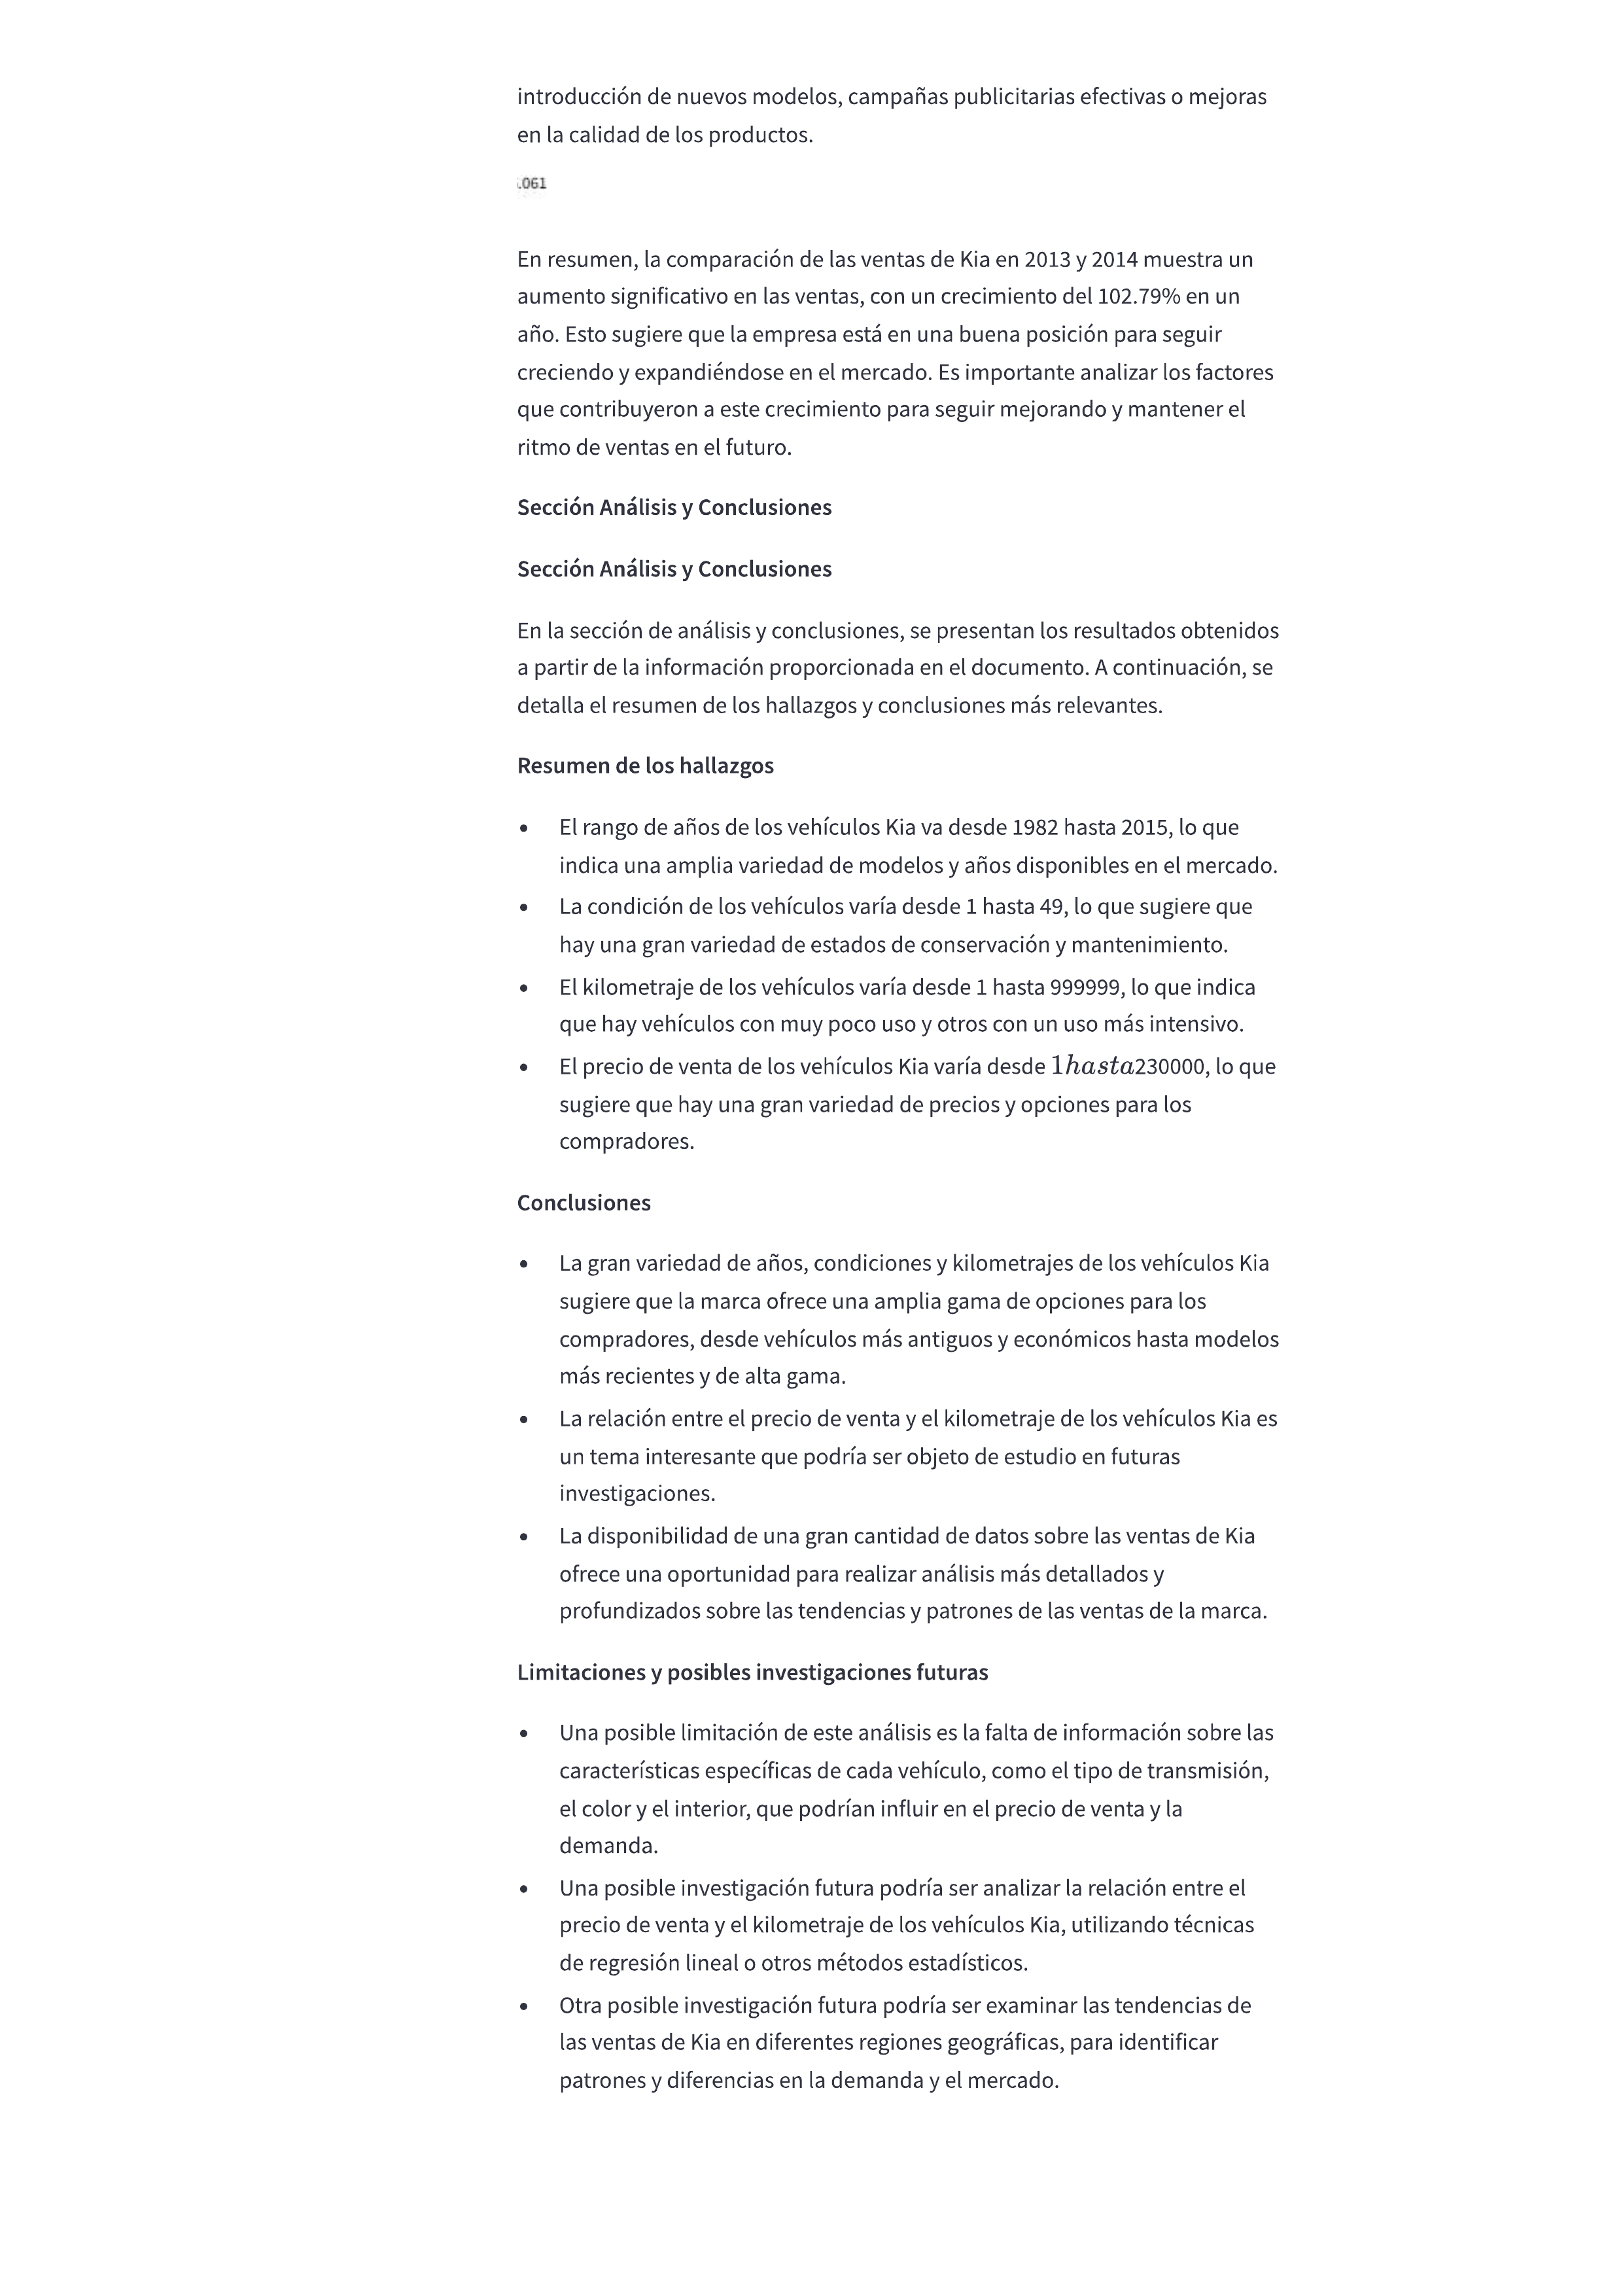
\includegraphics[height=\textheight]{reporte/5.png}
	\end{figure}
	\begin{figure}
		\centering
		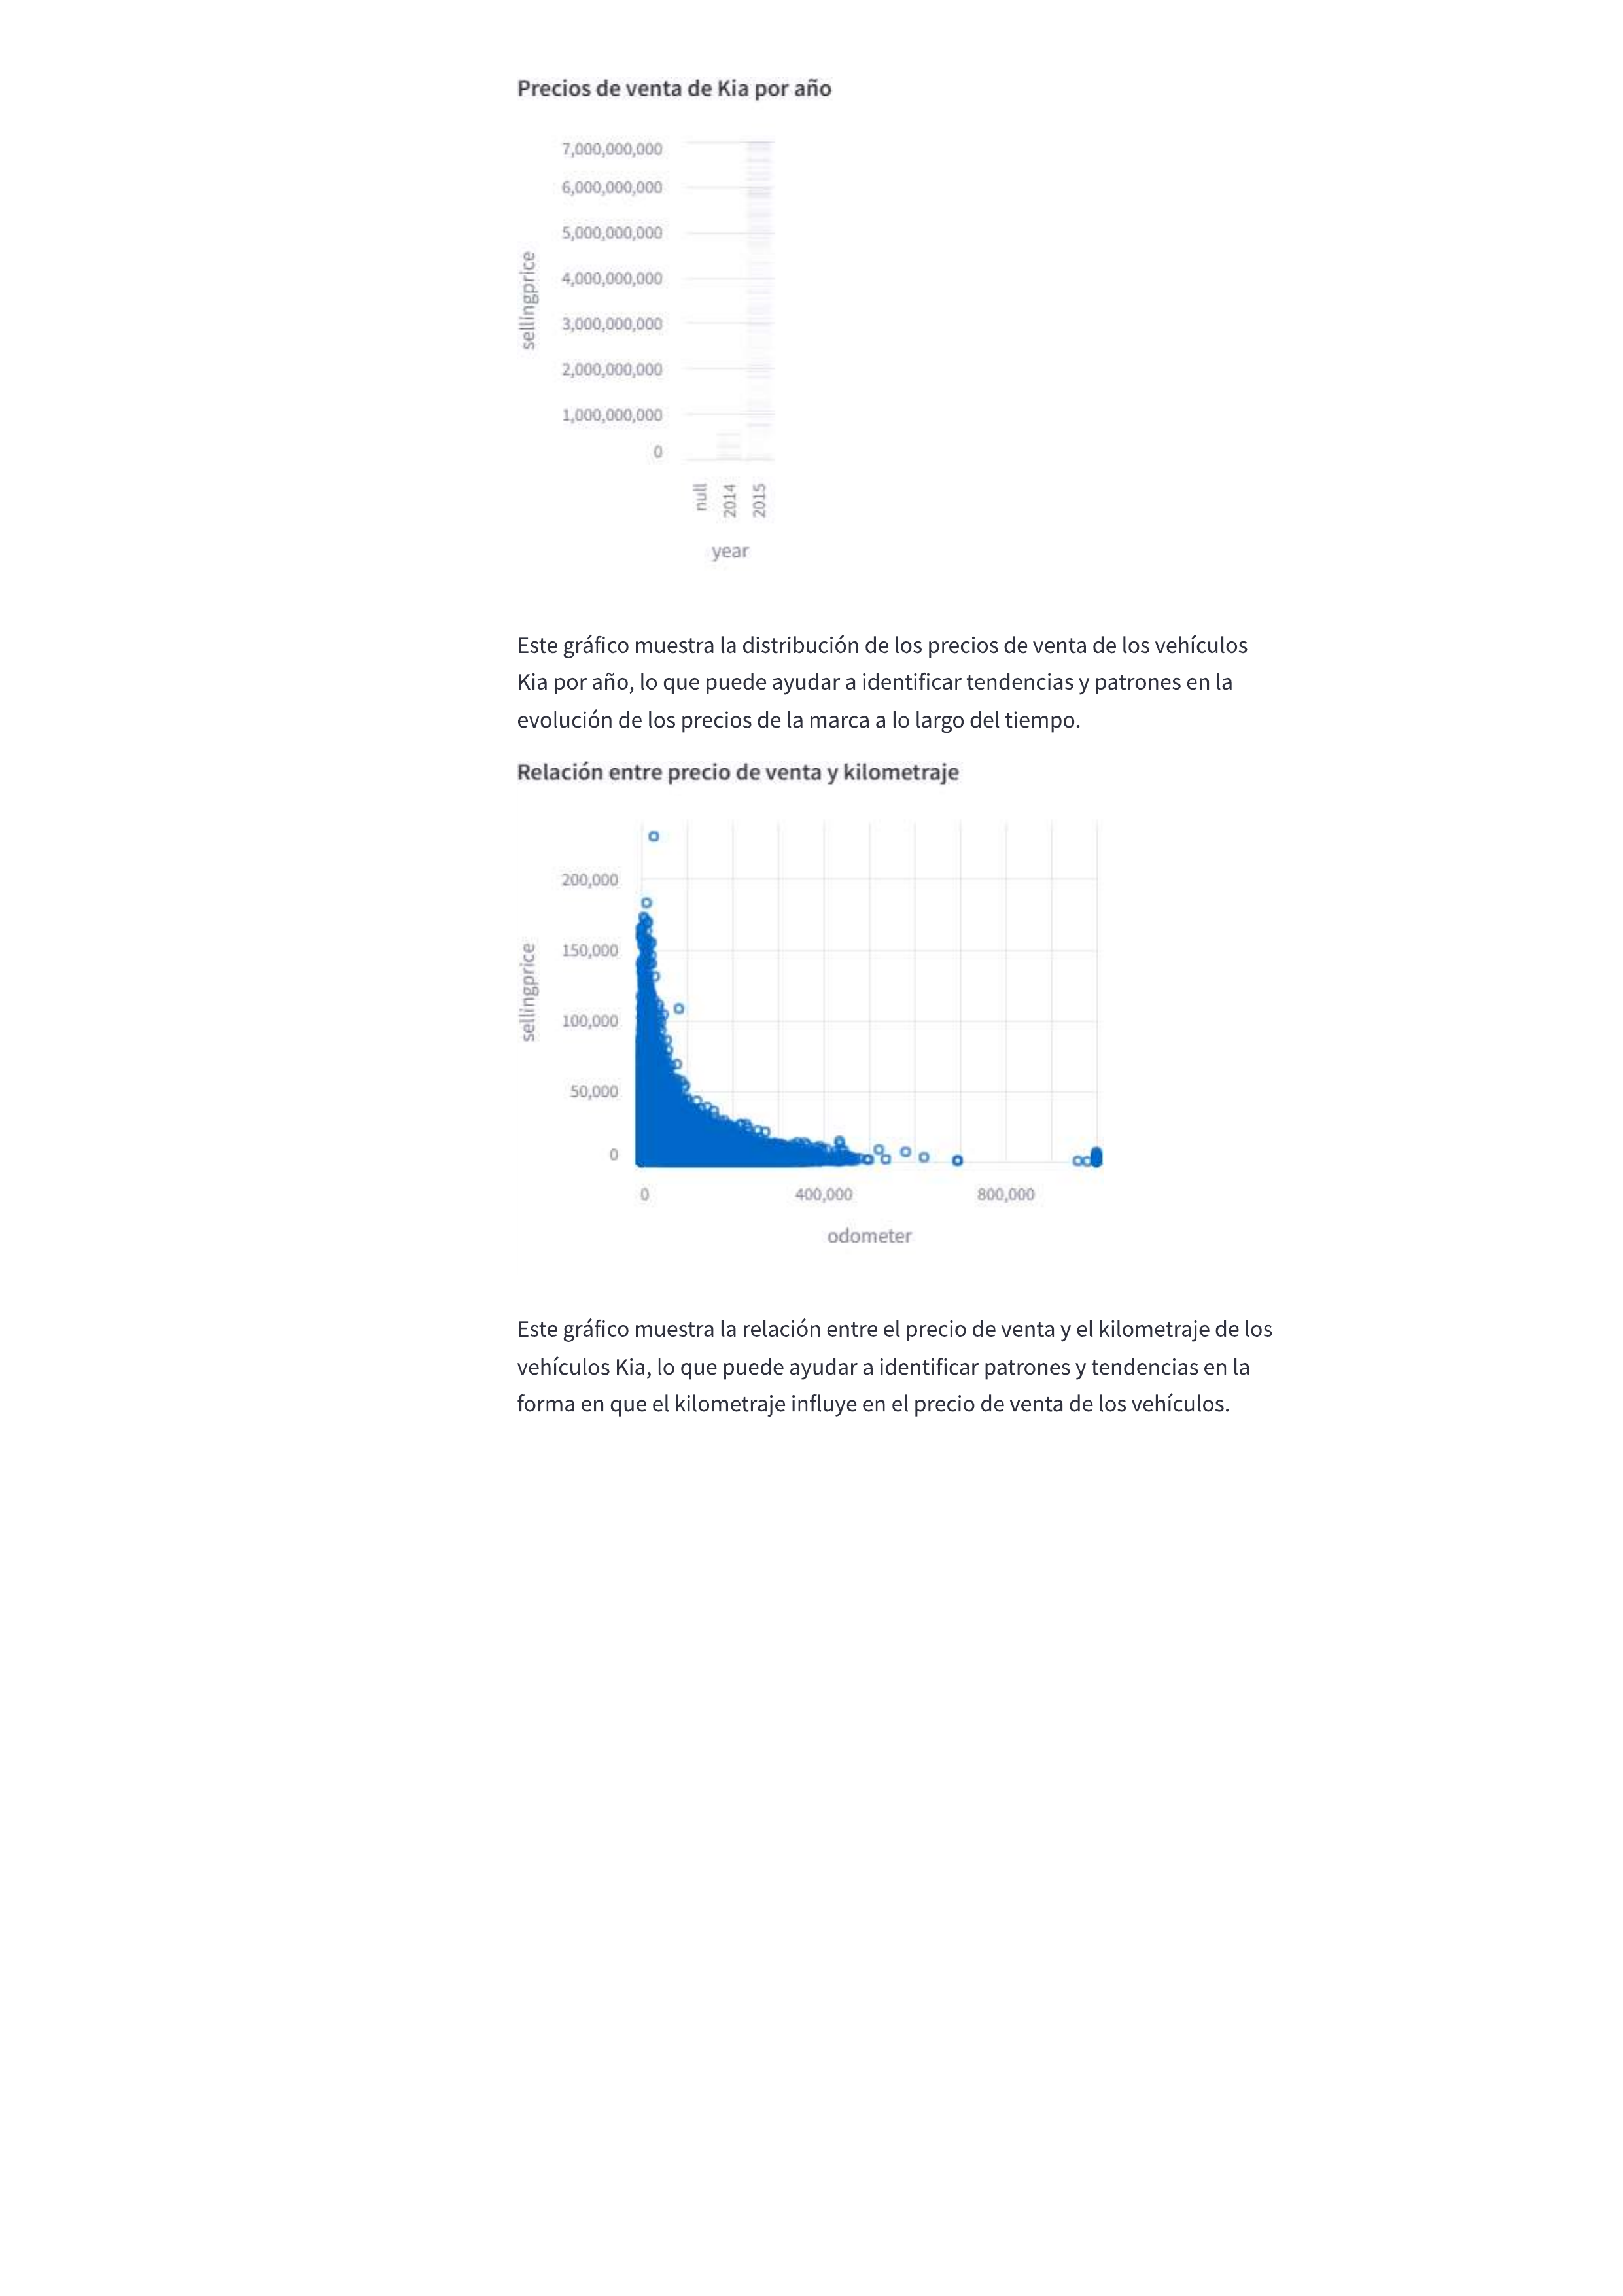
\includegraphics[height=\textheight]{reporte/6.png}
	\end{figure}
	
	
	\end{anexos}